\subsection{NGScopeClient}
	Once the data is gathered from the hardware it needs to be presented in a readable manner. We originally planned to build our own front-end application. Bryant has experience with front-end development and we did not know of any open source front ends that we liked. However, during Jeremy's hardware research, he spoke extensively with an engineer in the field who happened to mention ngscopeclient.org to him. When we saw it, we were sold. It is an open-source platform that works across OSX, Windows, and Linux. It can be interacted with using a C/C++ backend and it has beautiful graphics as shown in figure 2. It also has many built-in features for recognizing communication and data types that are very useful for our logic analysis. These features fit our application perfectly. 
	
		\begin{figure}[H]
		\centering
		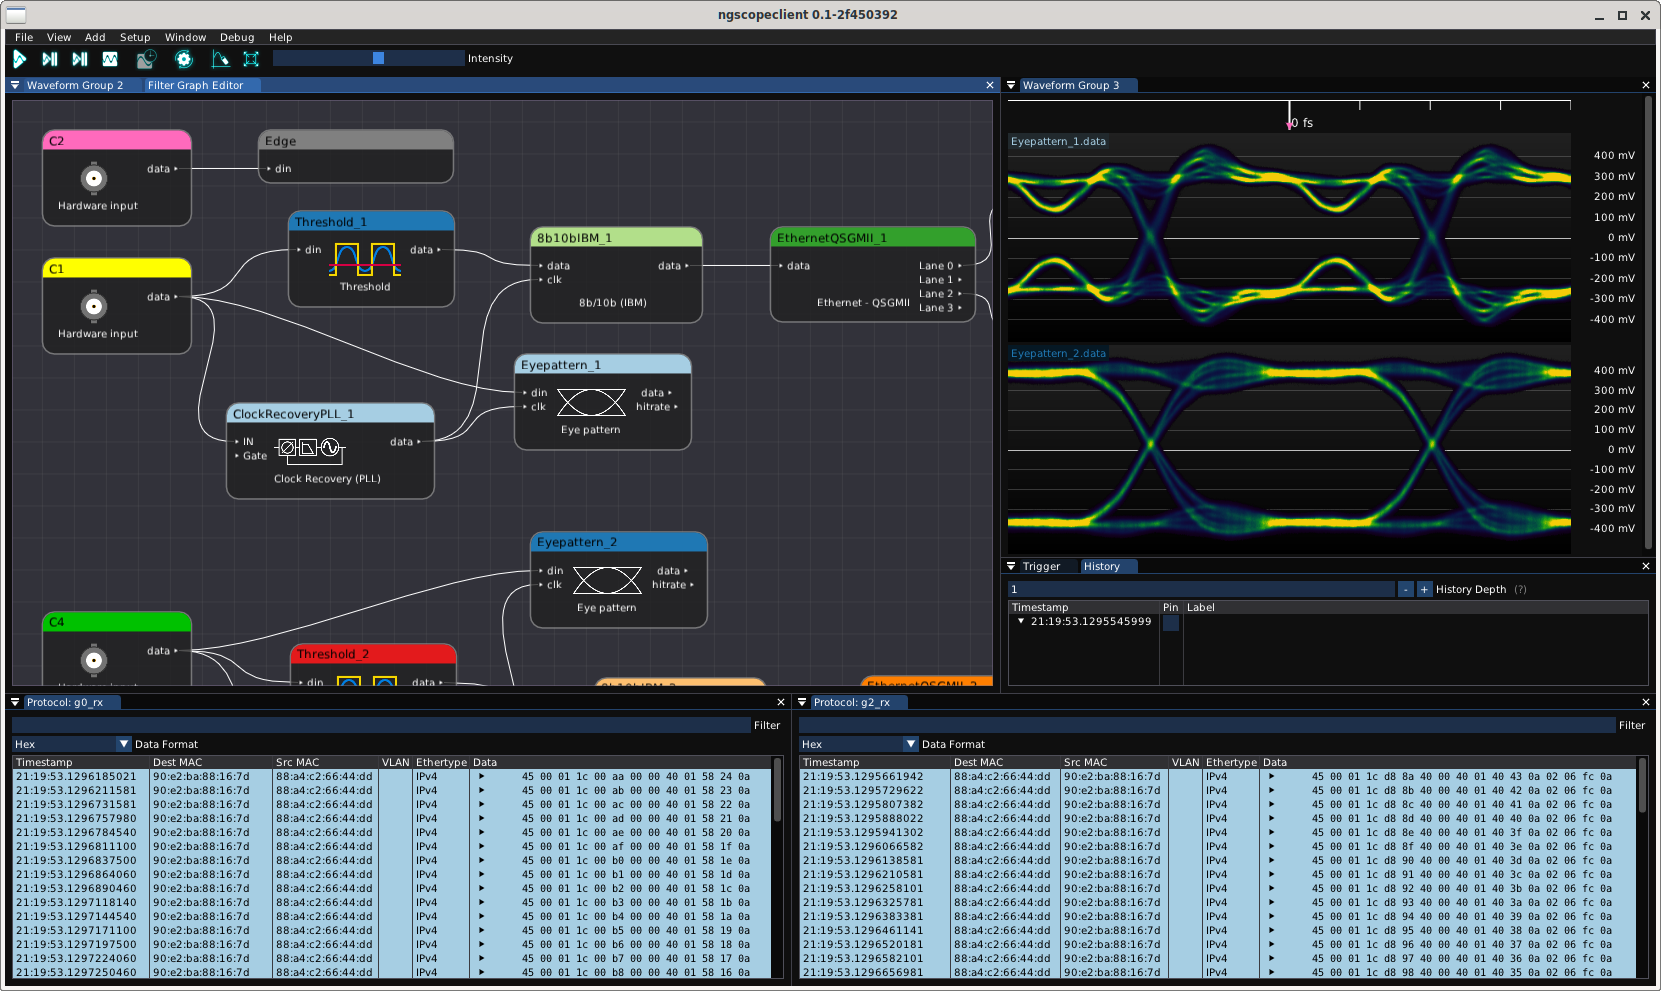
\includegraphics[width=0.8\linewidth]{images/ngscopeclient-intro.png}
		\caption{NGScopeClient Graphics \cite{ngscope_intro}}
		\label{fig:ngscope-client}
		\vspace{15px}
	\end{figure}
	

	‌